% This file was created by tikzplotlib v0.9.8.
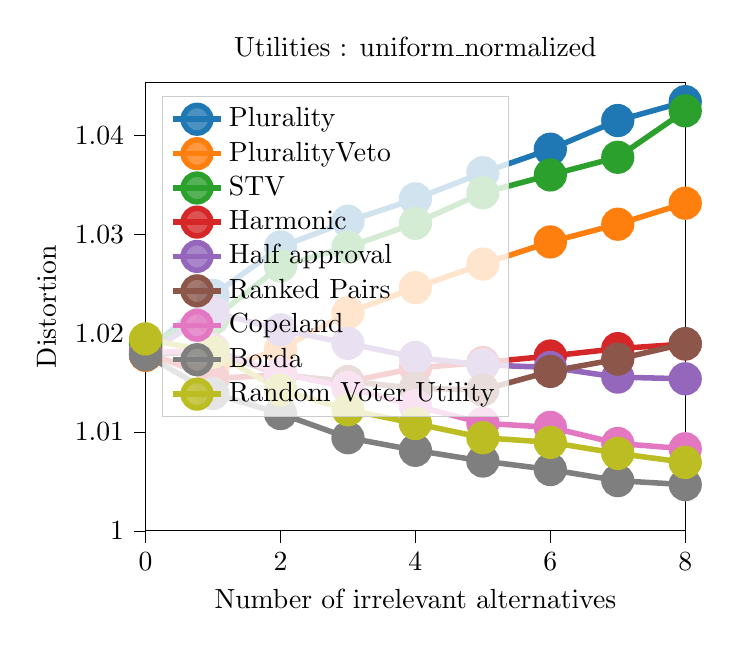
\begin{tikzpicture}

\definecolor{color0}{rgb}{0.12156862745098,0.466666666666667,0.705882352941177}
\definecolor{color1}{rgb}{1,0.498039215686275,0.0549019607843137}
\definecolor{color2}{rgb}{0.172549019607843,0.627450980392157,0.172549019607843}
\definecolor{color3}{rgb}{0.83921568627451,0.152941176470588,0.156862745098039}
\definecolor{color4}{rgb}{0.580392156862745,0.403921568627451,0.741176470588235}
\definecolor{color5}{rgb}{0.549019607843137,0.337254901960784,0.294117647058824}
\definecolor{color6}{rgb}{0.890196078431372,0.466666666666667,0.76078431372549}
\definecolor{color7}{rgb}{0.737254901960784,0.741176470588235,0.133333333333333}

\begin{axis}[
legend cell align={left},
legend style={
  fill opacity=0.8,
  draw opacity=1,
  text opacity=1,
  at={(0.03,0.97)},
  anchor=north west,
  draw=white!80!black
},
tick align=outside,
tick pos=left,
title={Utilities : uniform\_normalized},
x grid style={white!69.0196078431373!black},
xlabel={Number of irrelevant alternatives},
xmin=0, xmax=8,
xtick style={color=black},
y grid style={white!69.0196078431373!black},
ylabel={Distortion},
ymin=1, ymax=1.04537131557795,
ytick style={color=black}
]
\addplot [line width=2pt, color0, mark=*, mark size=5, mark options={solid}]
table {%
0 1.01809517873068
1 1.02383529100851
2 1.02873506027711
3 1.0313243528522
4 1.03359584325882
5 1.03624052063449
6 1.03862114008722
7 1.04151898886932
8 1.04343327275173
};
\addlegendentry{Plurality}
\addplot [line width=2pt, color1, mark=*, mark size=5, mark options={solid}]
table {%
0 1.01775123453029
1 1.01618638999177
2 1.01839417717616
3 1.02207157906109
4 1.0246128958258
5 1.0269907118042
6 1.02923515300153
7 1.03102890218125
8 1.03315558892466
};
\addlegendentry{PluralityVeto}
\addplot [line width=2pt, color2, mark=*, mark size=5, mark options={solid}]
table {%
0 1.01897992269222
1 1.02147450293511
2 1.02678826258995
3 1.02870939338639
4 1.03112583156506
5 1.03420199869228
6 1.03601489506272
7 1.03780291782111
8 1.04250233586205
};
\addlegendentry{STV}
\addplot [line width=2pt, color3, mark=*, mark size=5, mark options={solid}]
table {%
0 1.01811124306613
1 1.01541544257654
2 1.01579101201639
3 1.01507769113186
4 1.01648430441795
5 1.01703288635149
6 1.01768953615004
7 1.01843850315235
8 1.01890609203886
};
\addlegendentry{Harmonic}
\addplot [line width=2pt, color4, mark=*, mark size=5, mark options={solid}]
table {%
0 1.01789962415541
1 1.02213677173556
2 1.02034628668573
3 1.01897090869627
4 1.01754701345398
5 1.0167918148603
6 1.01653400150144
7 1.01555451238483
8 1.01538372302651
};
\addlegendentry{Half approval}
\addplot [line width=2pt, color5, mark=*, mark size=5, mark options={solid}]
table {%
0 1.01784733942526
1 1.01815197954205
2 1.01578859367271
3 1.01511028835828
4 1.01443481343589
5 1.01425812787123
6 1.01613238676683
7 1.01737307091767
8 1.01894332577351
};
\addlegendentry{Ranked Pairs}
\addplot [line width=2pt, color6, mark=*, mark size=5, mark options={solid}]
table {%
0 1.01797890827569
1 1.01834632954798
2 1.01591989906934
3 1.01451346214966
4 1.01265439487108
5 1.01089247226789
6 1.01047237783475
7 1.00884298427535
8 1.00830313287649
};
\addlegendentry{Copeland}
\addplot [line width=2pt, white!49.8039215686275!black, mark=*, mark size=5, mark options={solid}]
table {%
0 1.01782488261146
1 1.01389492617397
2 1.01186565429865
3 1.00942204295017
4 1.00814715178601
5 1.00706060093016
6 1.00619891959946
7 1.00507664226732
8 1.00467241622725
};
\addlegendentry{Borda}
\addplot [line width=2pt, color7, mark=*, mark size=5, mark options={solid}]
table {%
0 1.01942214154774
1 1.01807558438033
2 1.01425614934777
3 1.01225127731025
4 1.0108554539765
5 1.00942334661623
6 1.00895143261938
7 1.0078335885773
8 1.00692257958315
};
\addlegendentry{Random Voter Utility}
\end{axis}

\end{tikzpicture}
